\documentclass{beamer}
\usepackage{amsmath}
\usepackage{amsfonts}
\usepackage{amssymb}
\usepackage{polski}

\usetheme{Warsaw}
\usefonttheme[onlymath]{serif}

\usepackage{animate}
\usepackage{caption}
\usepackage{xcolor}

\usepackage{graphicx}
\usepackage{booktabs}
\usepackage{tabularx}
\usepackage{overpic}
\renewcommand{\arraystretch}{1.5}
\beamertemplatenavigationsymbolsempty

\usepackage[backend=biber,natbib=true]{biblatex}
\usepackage{aas_macros}
\addbibresource{bibliography.bib}
\renewcommand*{\bibfont}{\scriptsize}

\title{Być albo nie być czarną dziurą}
\author[F. Hansdorfer \and J. Winiarczyk \and Ł. Parda
\and T. Gruss]{Franciszek Hansdorfer \and Jacek Winiarczyk \and Łukasz Parda
\and Tomasz Gruss\\{\small Opiekun projektu: dr hab. Radosław Poleski}}
\date{\today}

\begin{document}

\begin{frame}
    \titlepage
\end{frame}
\section{Wprowadzenie do soczewkowania grawitacyjnego}
\subsection{Soczewkowanie grawitacyjne}

\begin{frame}
    \begin{columns}
        \begin{column}{0.5\linewidth}
            \begin{itemize}
                \item Ogólna teoria względności $\implies$
                \item Masa zakrzywia czasoprzestrzeń $\implies$
                \item Światło idące w pobliżu masy jest odchylane $\implies$
                \item Obserwator widzi obiekty za zakrzywiającą masą w inny sposób $\implies$
                \item Soczewkowanie grawitacyjne
            \end{itemize}
        \end{column}
        \begin{column}{0.5\linewidth}
            \begin{figure}
                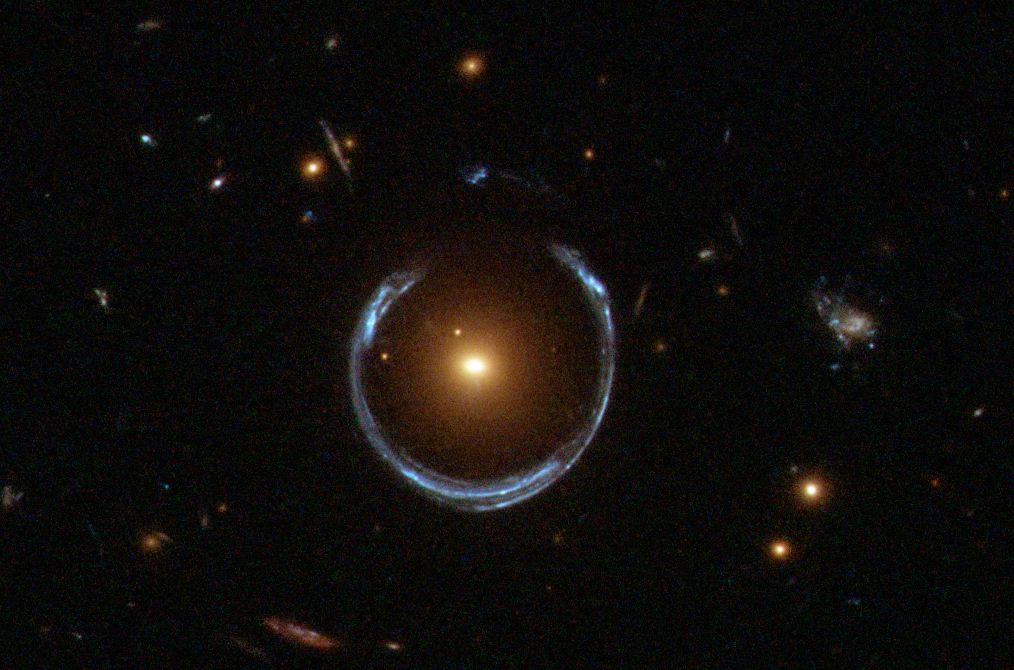
\includegraphics[width=\textwidth]{A_Horseshoe_Einstein_Ring_from_Hubble.jpeg}
                \caption*{\tiny{ESA/Hubble, NASA}}
            \end{figure}
        \end{column}
    \end{columns}
\end{frame}

\begin{frame}
    \begin{figure}
        \centering
        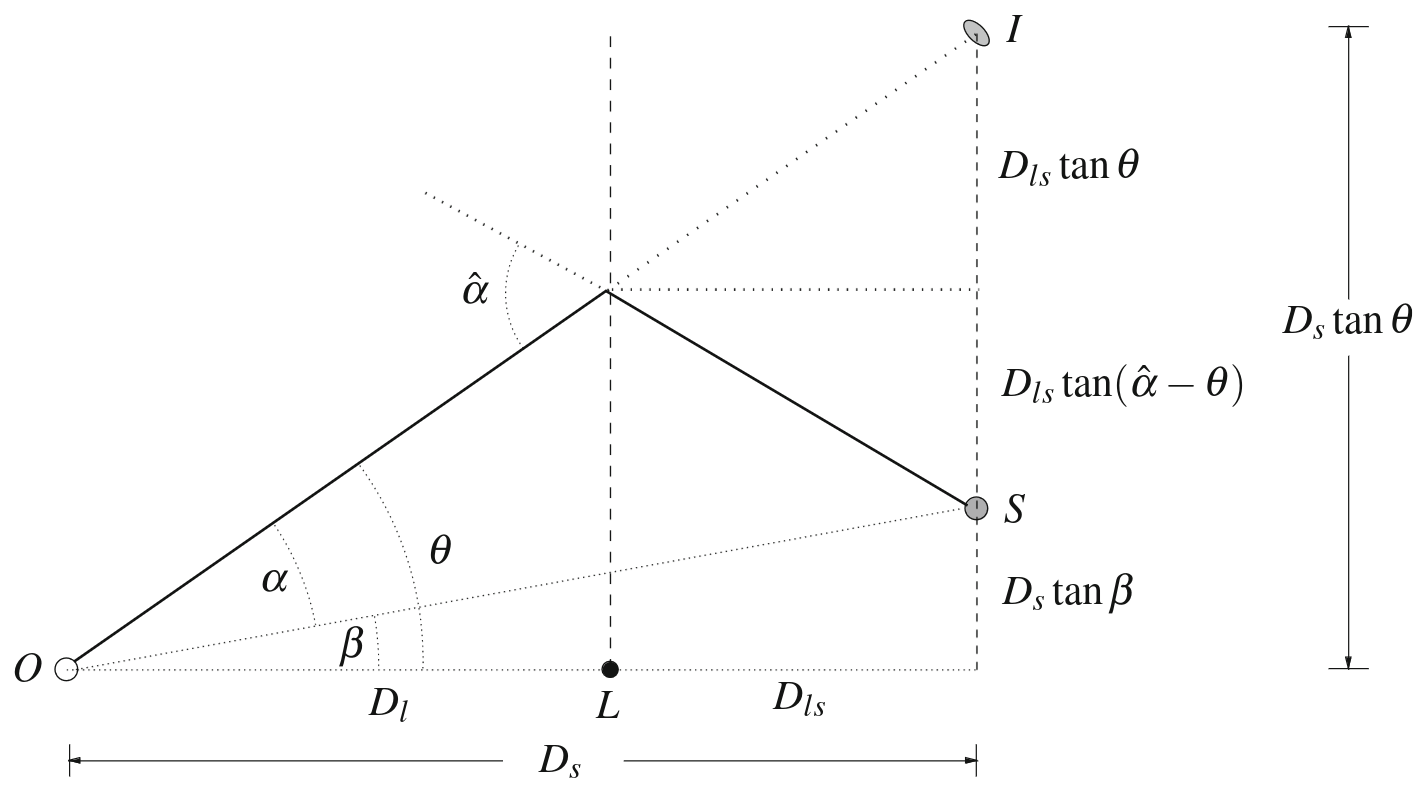
\includegraphics[width=0.6\textwidth]{Screenshot from 2024-06-10 13-41-41.png}
        \caption*{\tiny{Principles of Gravitational
                Lensing, Arthur B. Congdon, Charles R. Keeton \cite{Congdon2018}}}
    \end{figure}
    \textbf{Równanie soczewki}:
    \[\beta = \theta - \alpha(\theta)\]
    Dla punktowej masy mamy \cite{Schneider1992}:
    \[\theta_E = \sqrt{\frac{4GM}{c^2}\frac{D_s-D_l}{D_s D_l}}\]
\end{frame}

\subsection{Mikrosoczewkowanie}
\begin{frame}{Mikrosoczewkowanie}
    \begin{columns}
        \begin{column}{0.6\linewidth}
            \[M \sim M_{\odot}\]
            Na przykład dla $D_s = 8 \text{ kpc}$, $D_l = 4 \text{ kpc}$, $M = 1 M_{\odot}$:
            \[\theta_E = 0.32 \text{ mas}\]
            Dla $u = \frac{\beta}{\theta_E}$ wzmocnienie źródła określa wzór \cite{Schneider1992}:
            \[A(u) = \frac{u^2 + 2}{u \sqrt{u^2 + 4}}\]
            \[u(t) = \sqrt{u_0^2 + \left(\frac{t-t_0}{t_E}\right)^2}\]
        \end{column}
        \begin{column}{0.4\linewidth}
            \begin{figure}
                \centering
                \only<1>{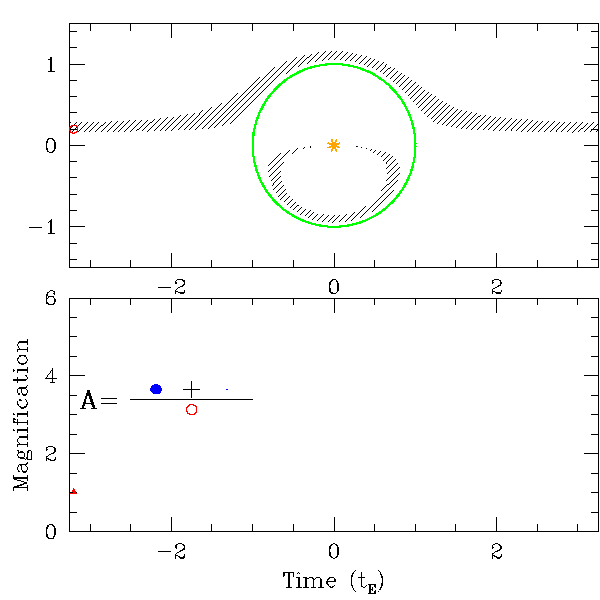
\includegraphics[width=\textwidth]{animation1/Scott_Gaudi_anim-0}}
                \only<2>{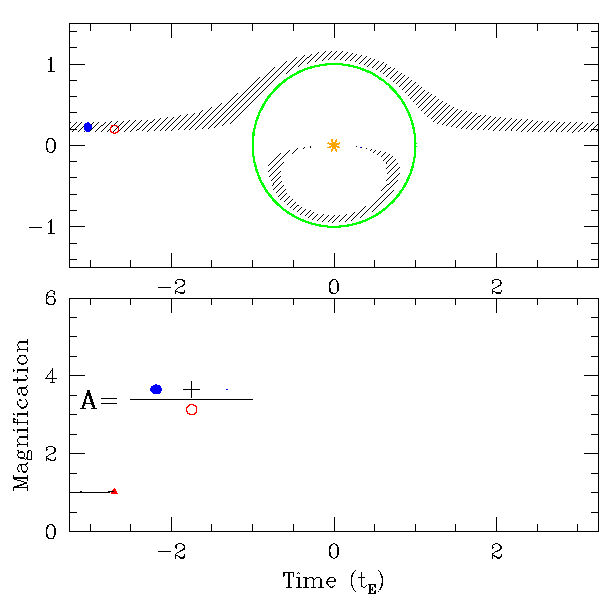
\includegraphics[width=\textwidth]{animation1/Scott_Gaudi_anim-5}}
                \only<3>{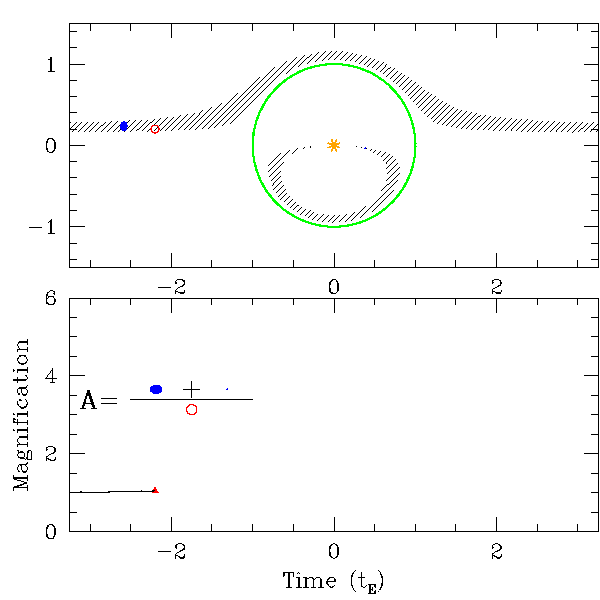
\includegraphics[width=\textwidth]{animation1/Scott_Gaudi_anim-10}}
                \only<4>{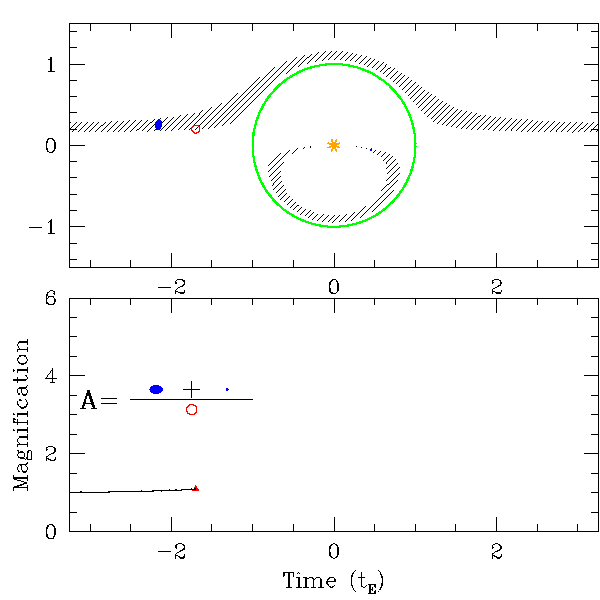
\includegraphics[width=\textwidth]{animation1/Scott_Gaudi_anim-15}}
                \only<5>{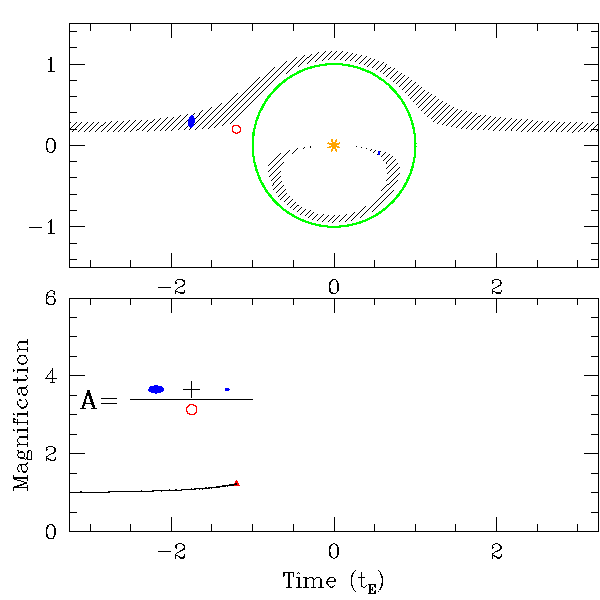
\includegraphics[width=\textwidth]{animation1/Scott_Gaudi_anim-20}}
                \only<6>{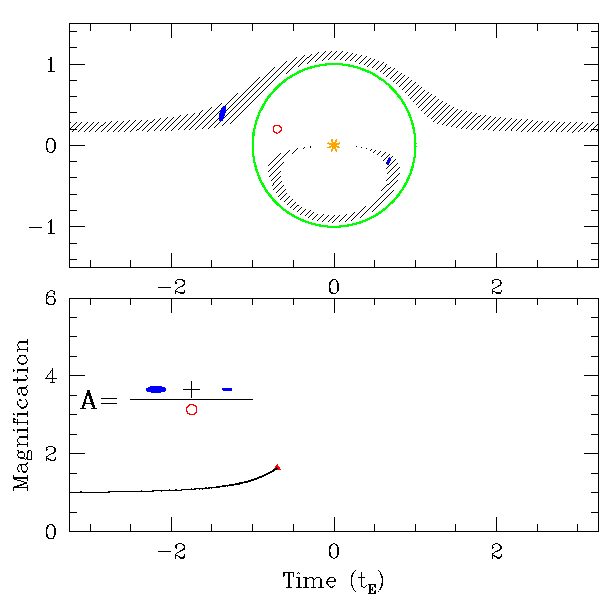
\includegraphics[width=\textwidth]{animation1/Scott_Gaudi_anim-25}}
                \only<7>{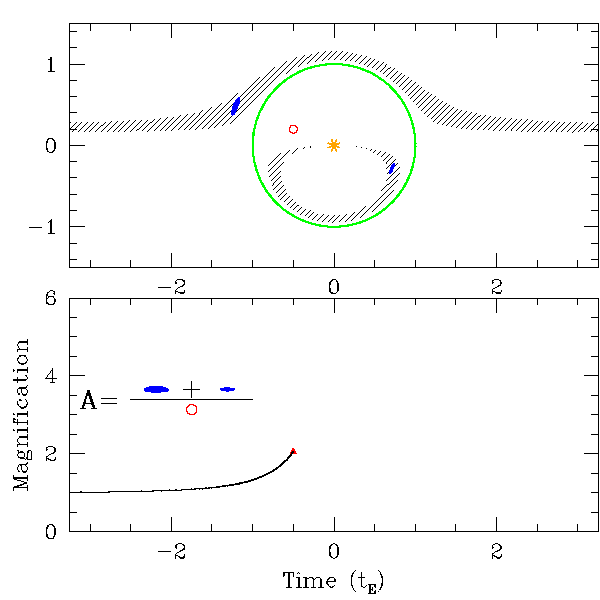
\includegraphics[width=\textwidth]{animation1/Scott_Gaudi_anim-27}}
                \only<8>{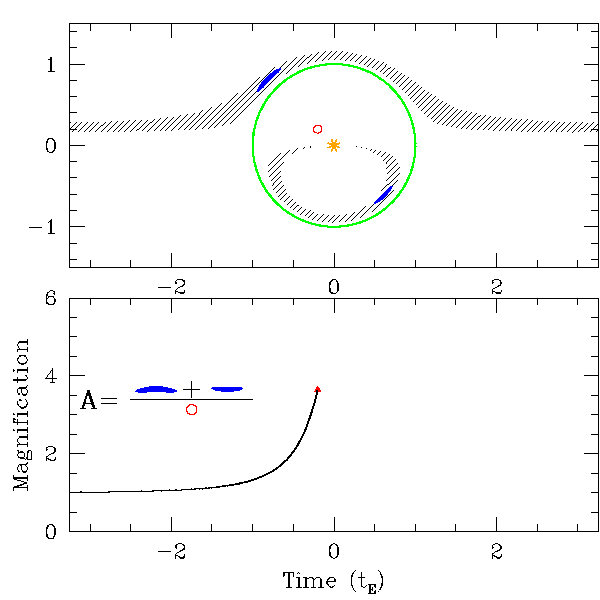
\includegraphics[width=\textwidth]{animation1/Scott_Gaudi_anim-30}}
                \only<9>{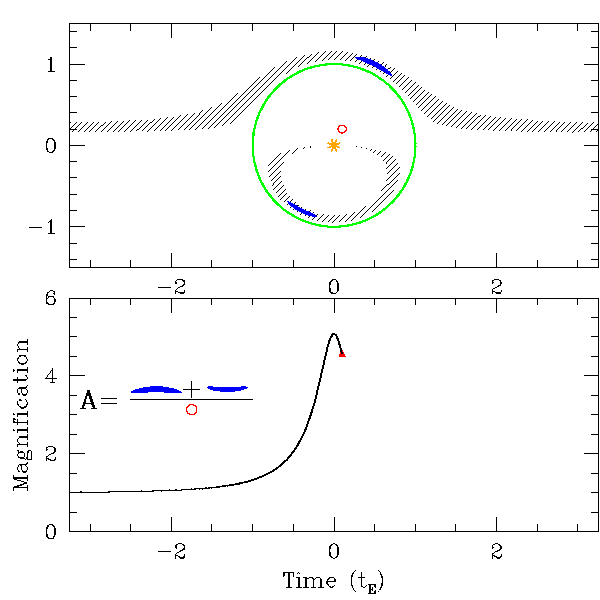
\includegraphics[width=\textwidth]{animation1/Scott_Gaudi_anim-33}}
                \only<10>{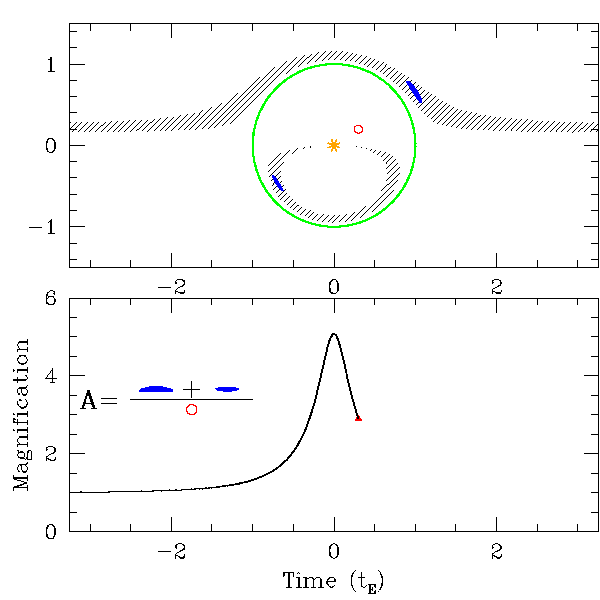
\includegraphics[width=\textwidth]{animation1/Scott_Gaudi_anim-35}}
                \only<11>{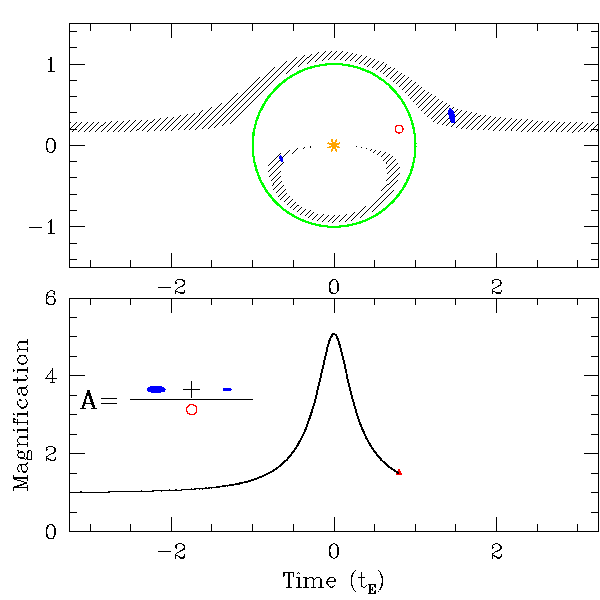
\includegraphics[width=\textwidth]{animation1/Scott_Gaudi_anim-40}}
                \only<12>{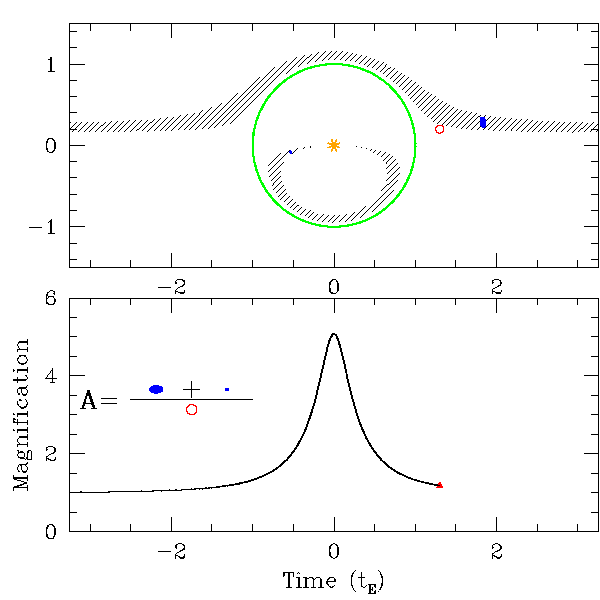
\includegraphics[width=\textwidth]{animation1/Scott_Gaudi_anim-45}}
                \only<13>{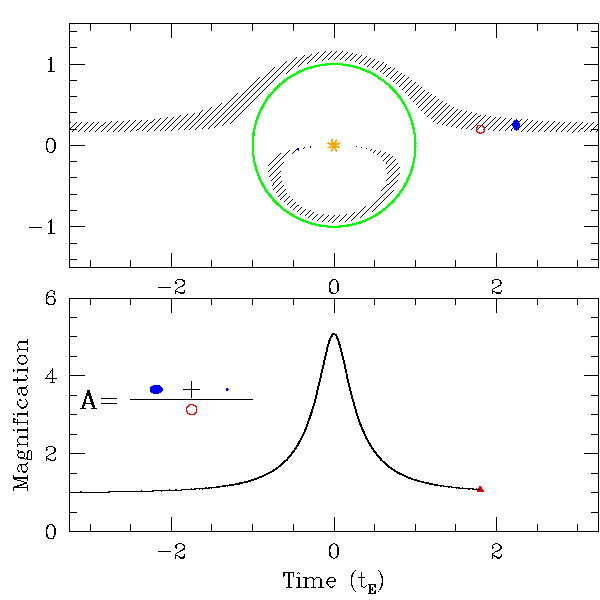
\includegraphics[width=\textwidth]{animation1/Scott_Gaudi_anim-50}}
                \only<14>{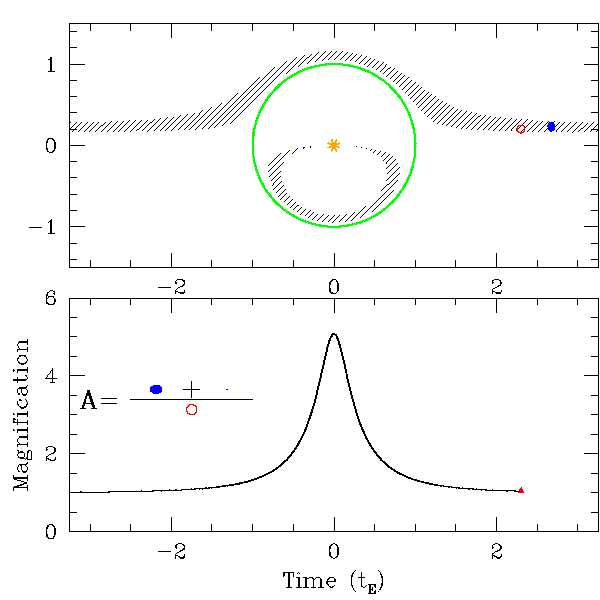
\includegraphics[width=\textwidth]{animation1/Scott_Gaudi_anim-55}}
                \only<15>{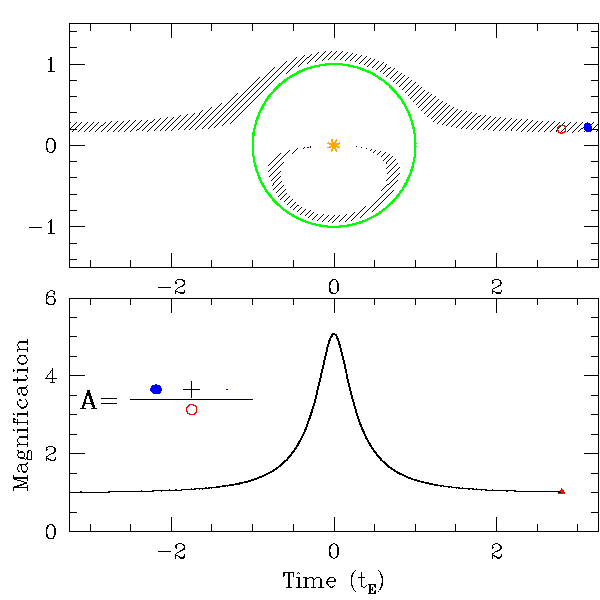
\includegraphics[width=\textwidth]{animation1/Scott_Gaudi_anim-60}}
                \only<16>{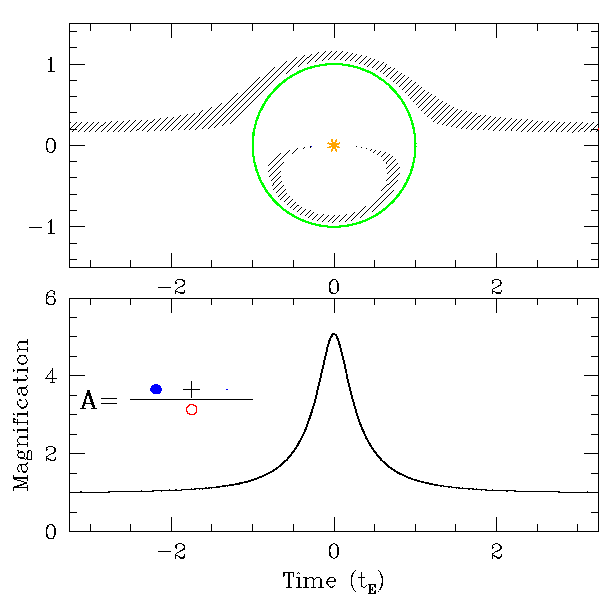
\includegraphics[width=\textwidth]{animation1/Scott_Gaudi_anim-65}}
                \caption*{\tiny{Animation by B.S. Gaudi - microlensing-source.org}}
            \end{figure}
        \end{column}
    \end{columns}

\end{frame}

\subsection{Odchylenia od modelu punktowego źródła i soczewki}

\begin{frame}{Paralaksa}
    \begin{columns}
        \begin{column}{0.4\linewidth}
            Dla $t_{\text{E}}>30 \text{ d}$ ruchu Ziemi wokół Słońca przestaje być pomijalny. Wtedy wzór na $u(t)$ jest bardziej skomplikowany.

        \end{column}

        \begin{column}{0.5\linewidth}
            \begin{figure}
                \centering
                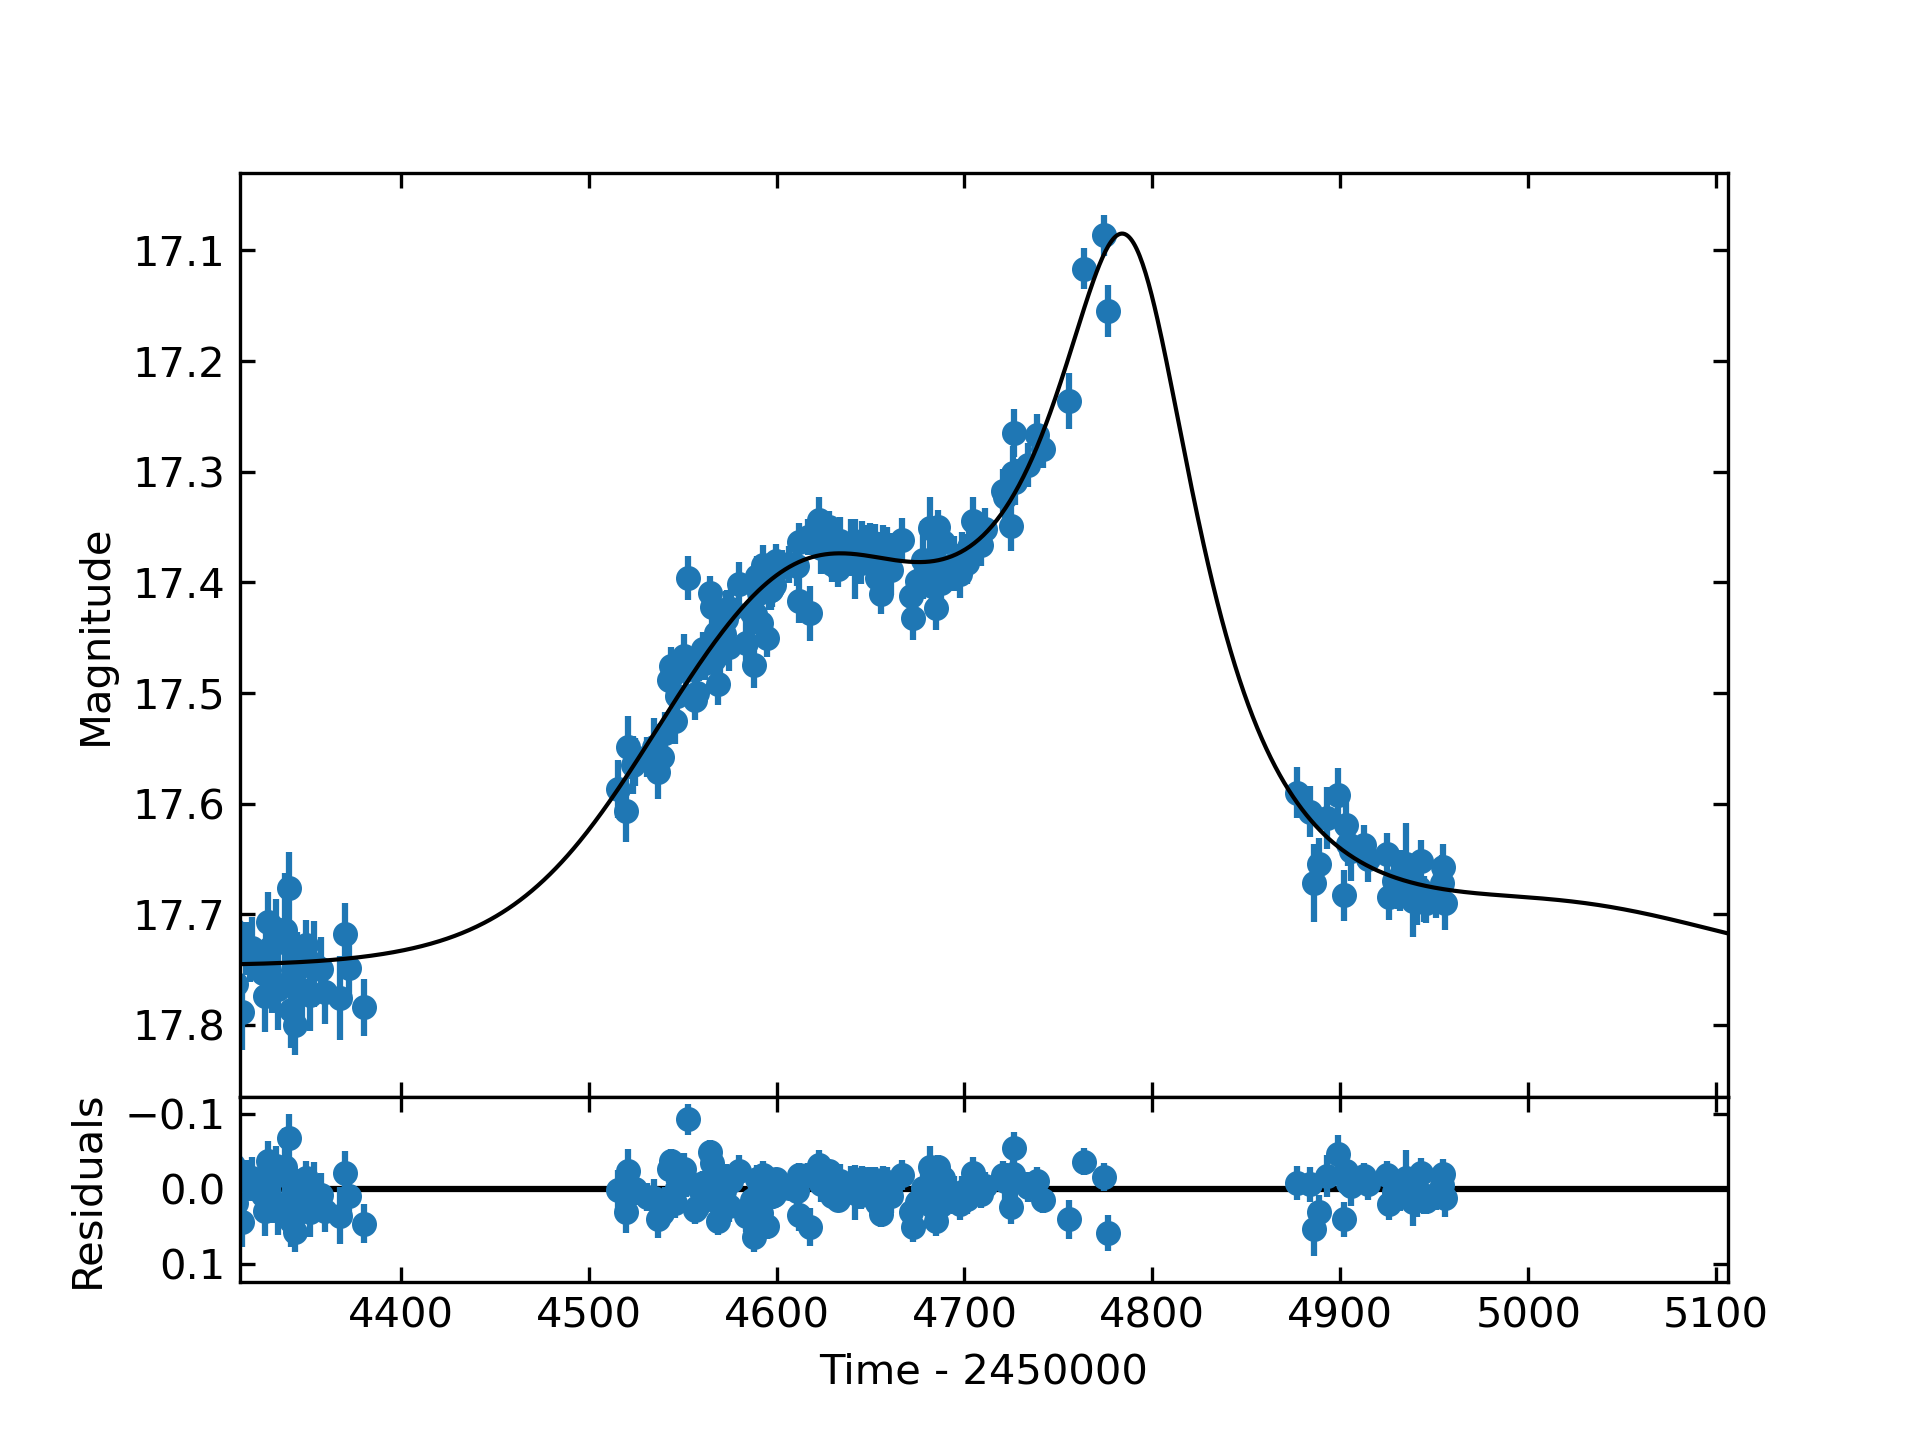
\includegraphics[width = \textwidth]{../sim30/parallax/png/PAR-20-noaver.dat-.png}
                \caption*{\tiny{PAR-20, $u_0<0$}}
            \end{figure}
        \end{column}
    \end{columns}

\end{frame}

\begin{frame}{Paralaksa}
    \vspace{-0.3cm}
    \begin{columns}
        \begin{column}{0.45\linewidth}
            \begin{figure}
                \centering
                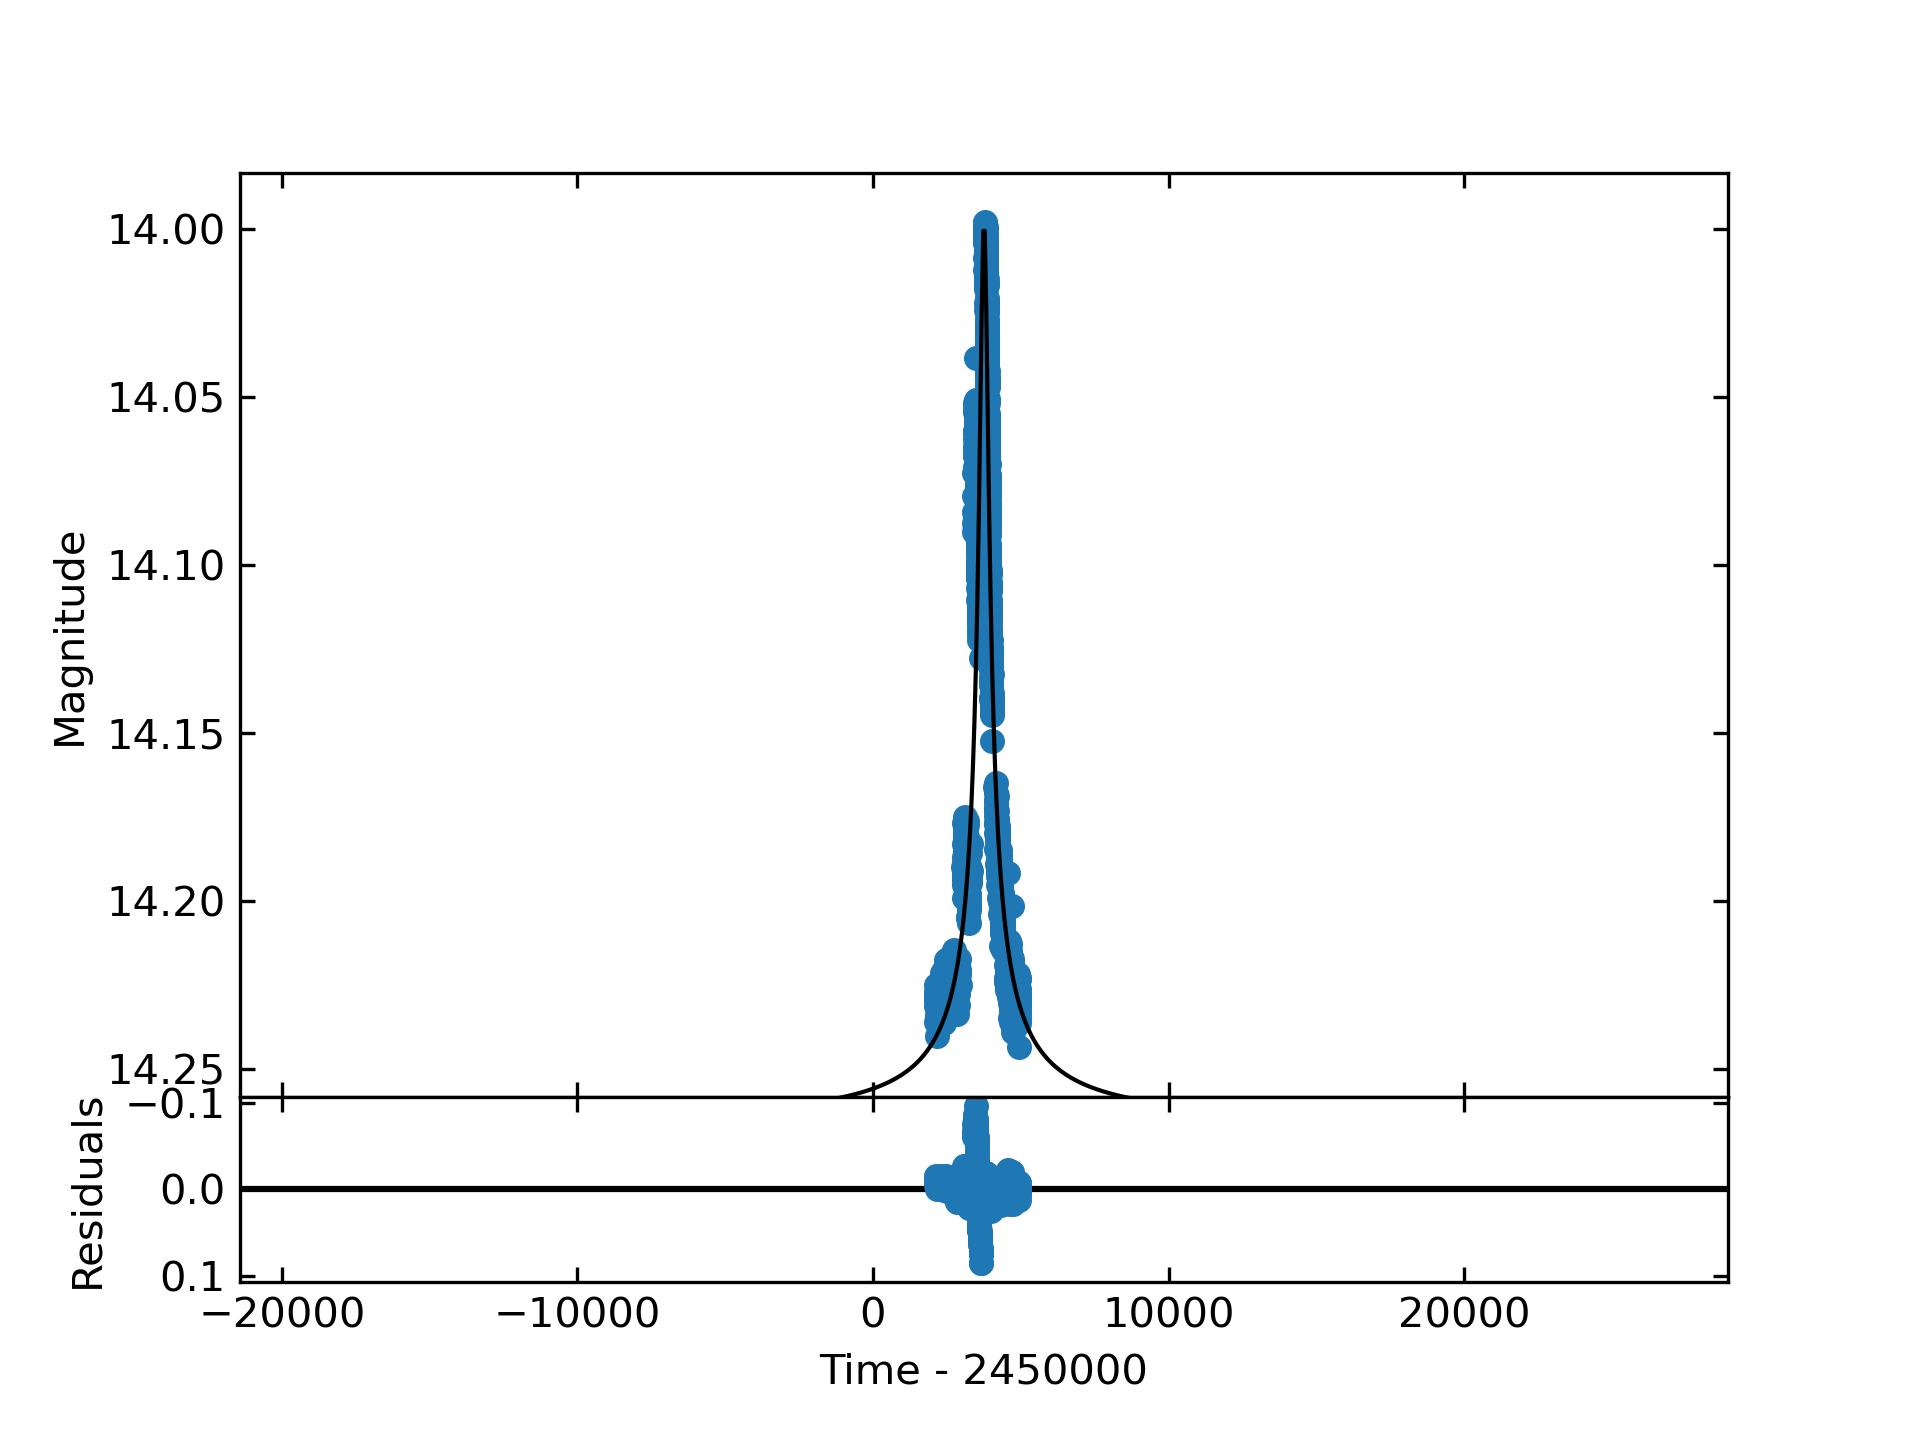
\includegraphics[width = \textwidth]{../sim30/nothing/png/PAR-01-noaver.dat.png}
                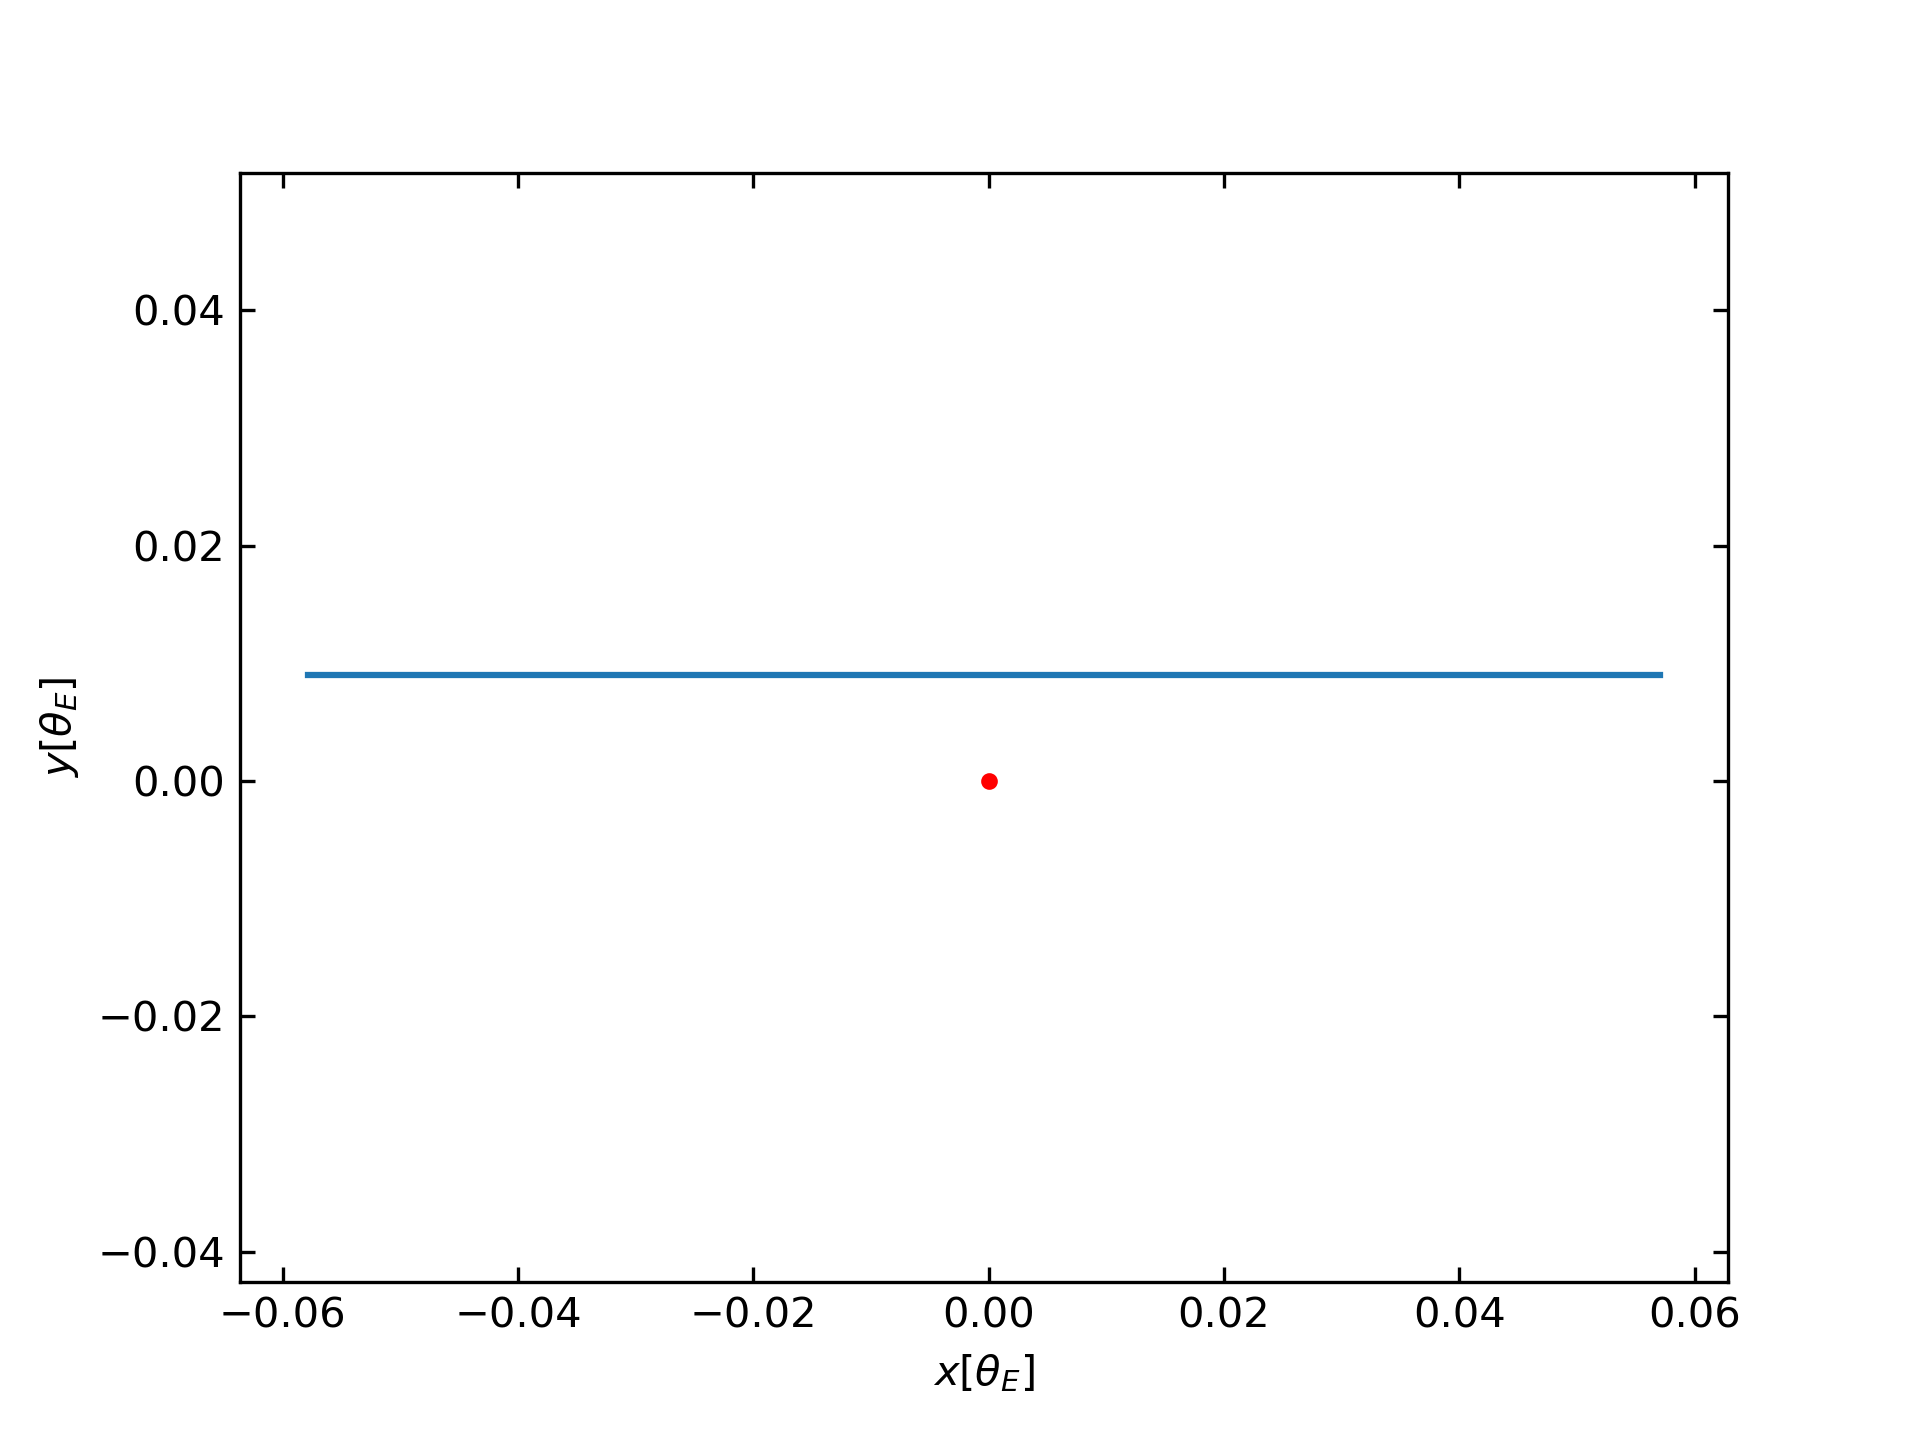
\includegraphics[width = \textwidth]{../sim30/nothing/png/PAR-01-noaver.dat.trj.png}

            \end{figure}
        \end{column}
    
        \begin{column}{0.45\linewidth}
            \begin{figure}
                \centering
                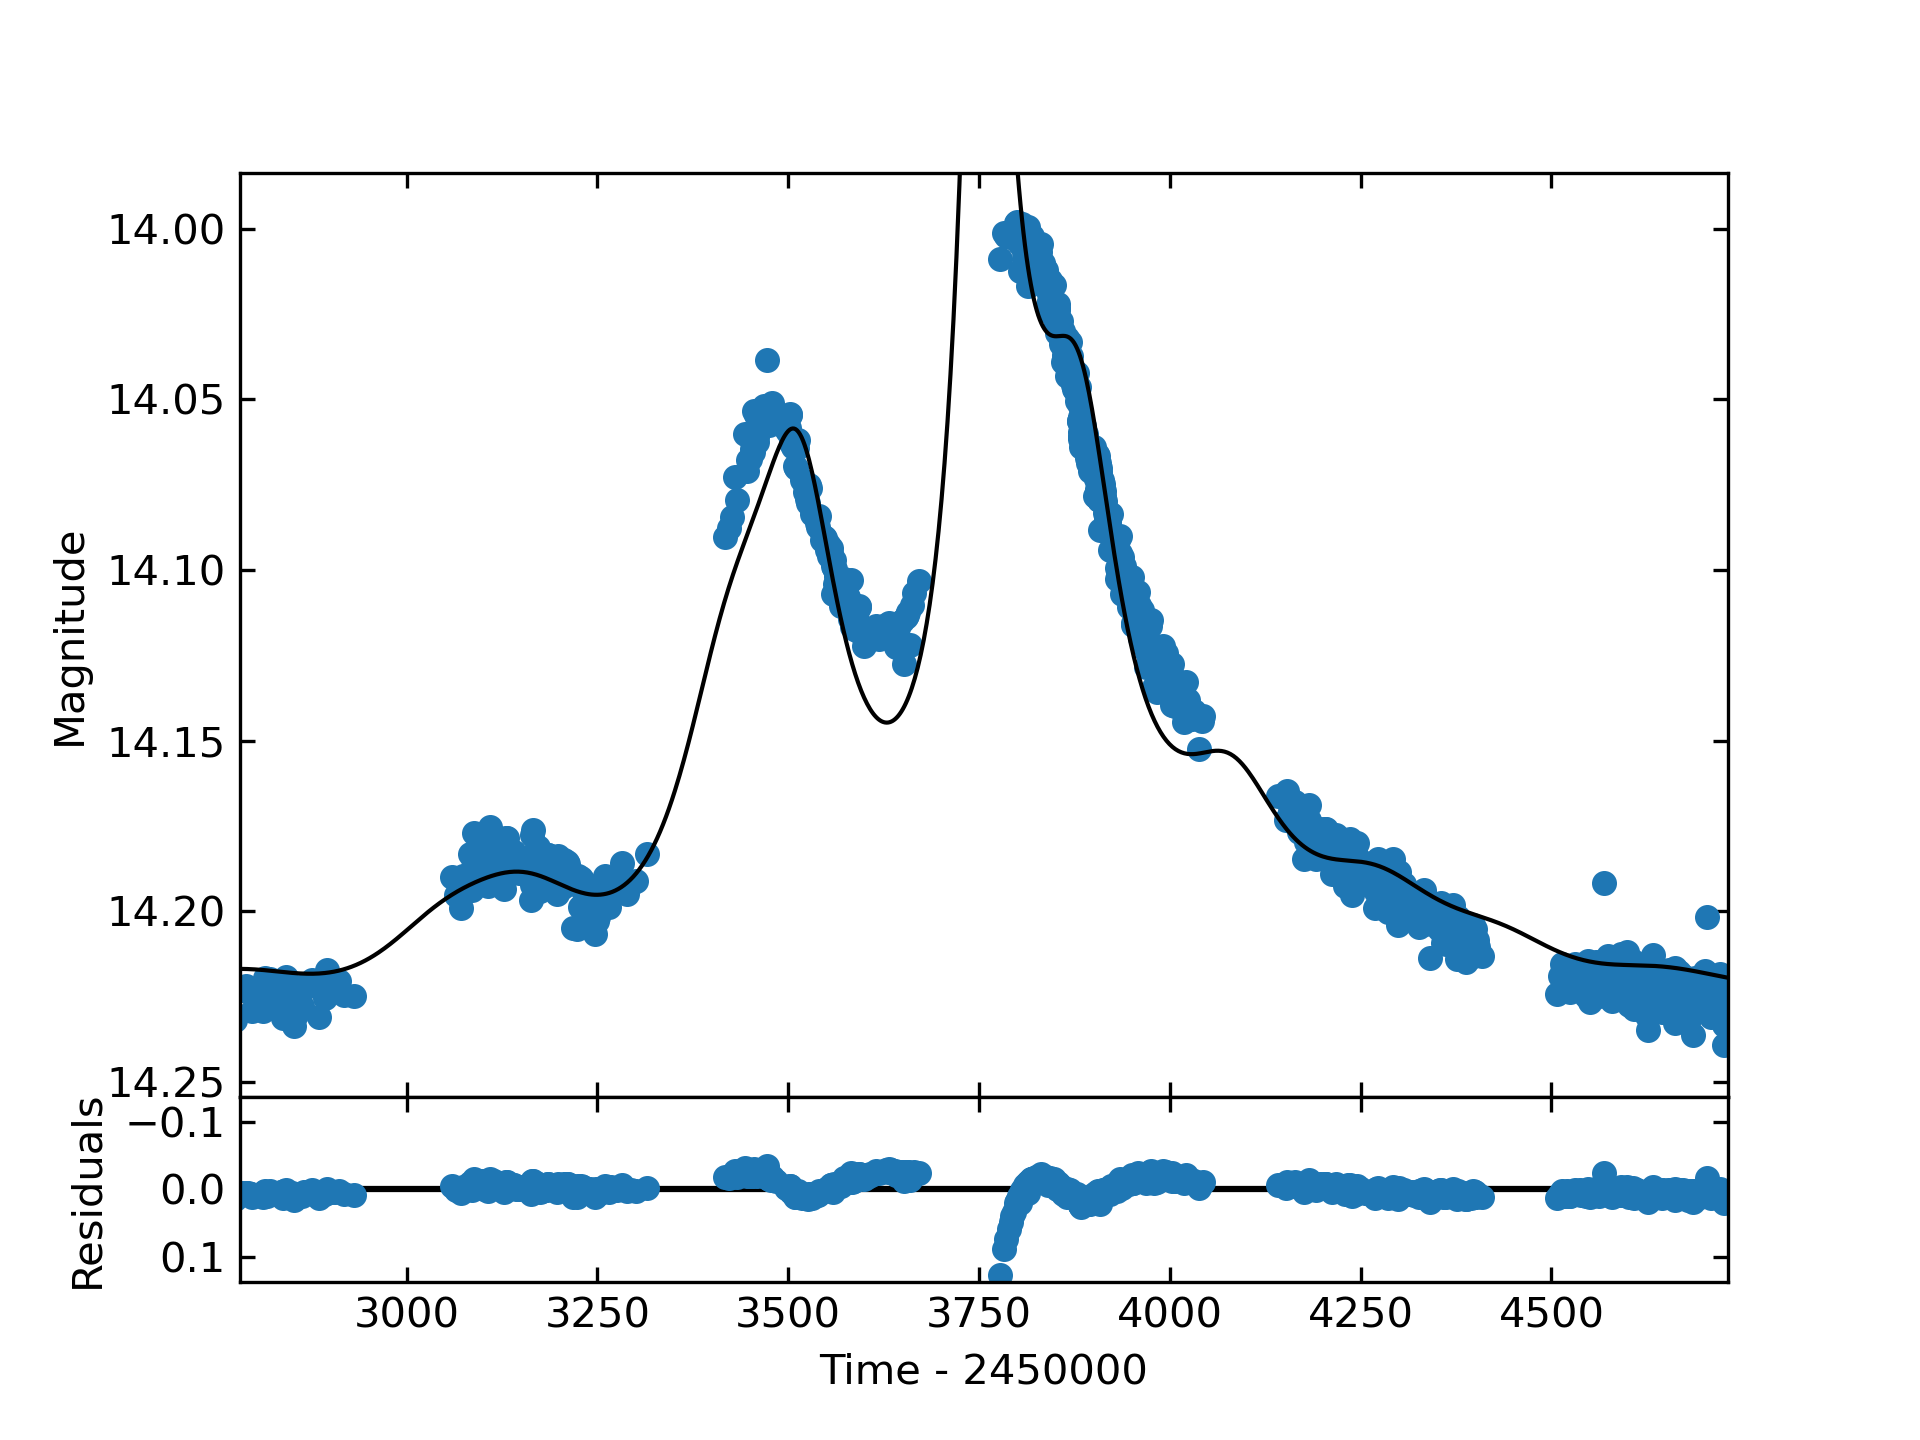
\includegraphics[width = \textwidth]{../sim30/parallax/png/PAR-01-noaver.dat-.png}
                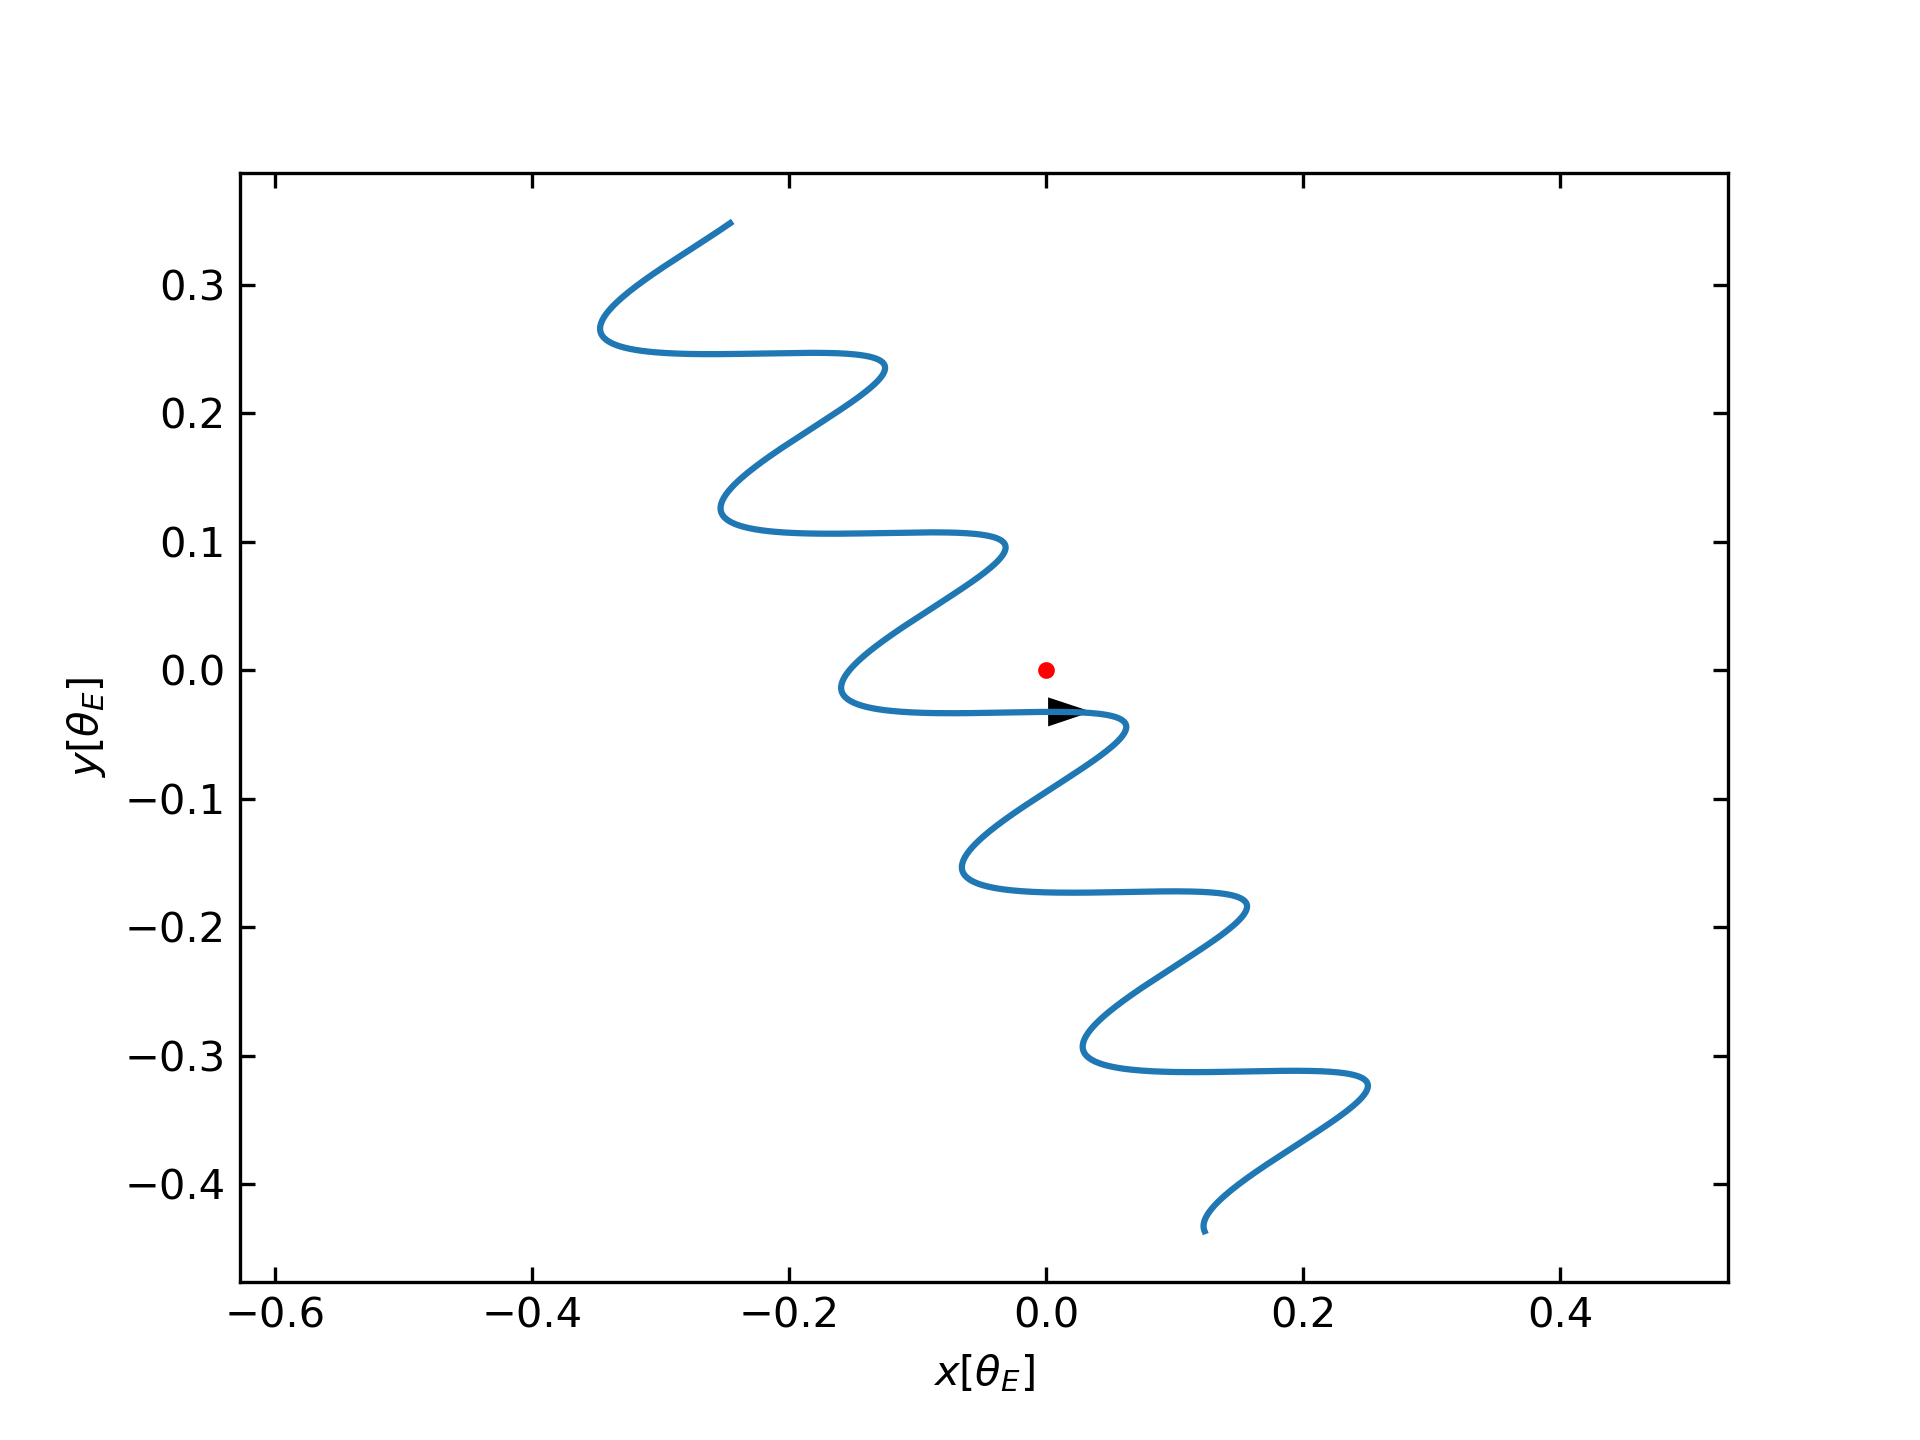
\includegraphics[width = \textwidth]{../sim30/parallax/png/PAR-01-noaver.dat-.trj.png}

            \end{figure}
        \end{column}
    \end{columns}

\end{frame}

\begin{frame}{Xallarap}
    \begin{columns}
        \begin{column}{0.5\linewidth}
            Jeżeli źródło jest częścią układu podwójnego, to jego ruch orbitalny może mieć znaczący wpływ na parametr $u(t)$.
            To zjawisko nosi nazwę xallarap (parallax od tyłu) \cite{Xallarap_paper}.
        \end{column}
        \begin{column}{0.5\linewidth}
            \begin{figure}
                \centering
                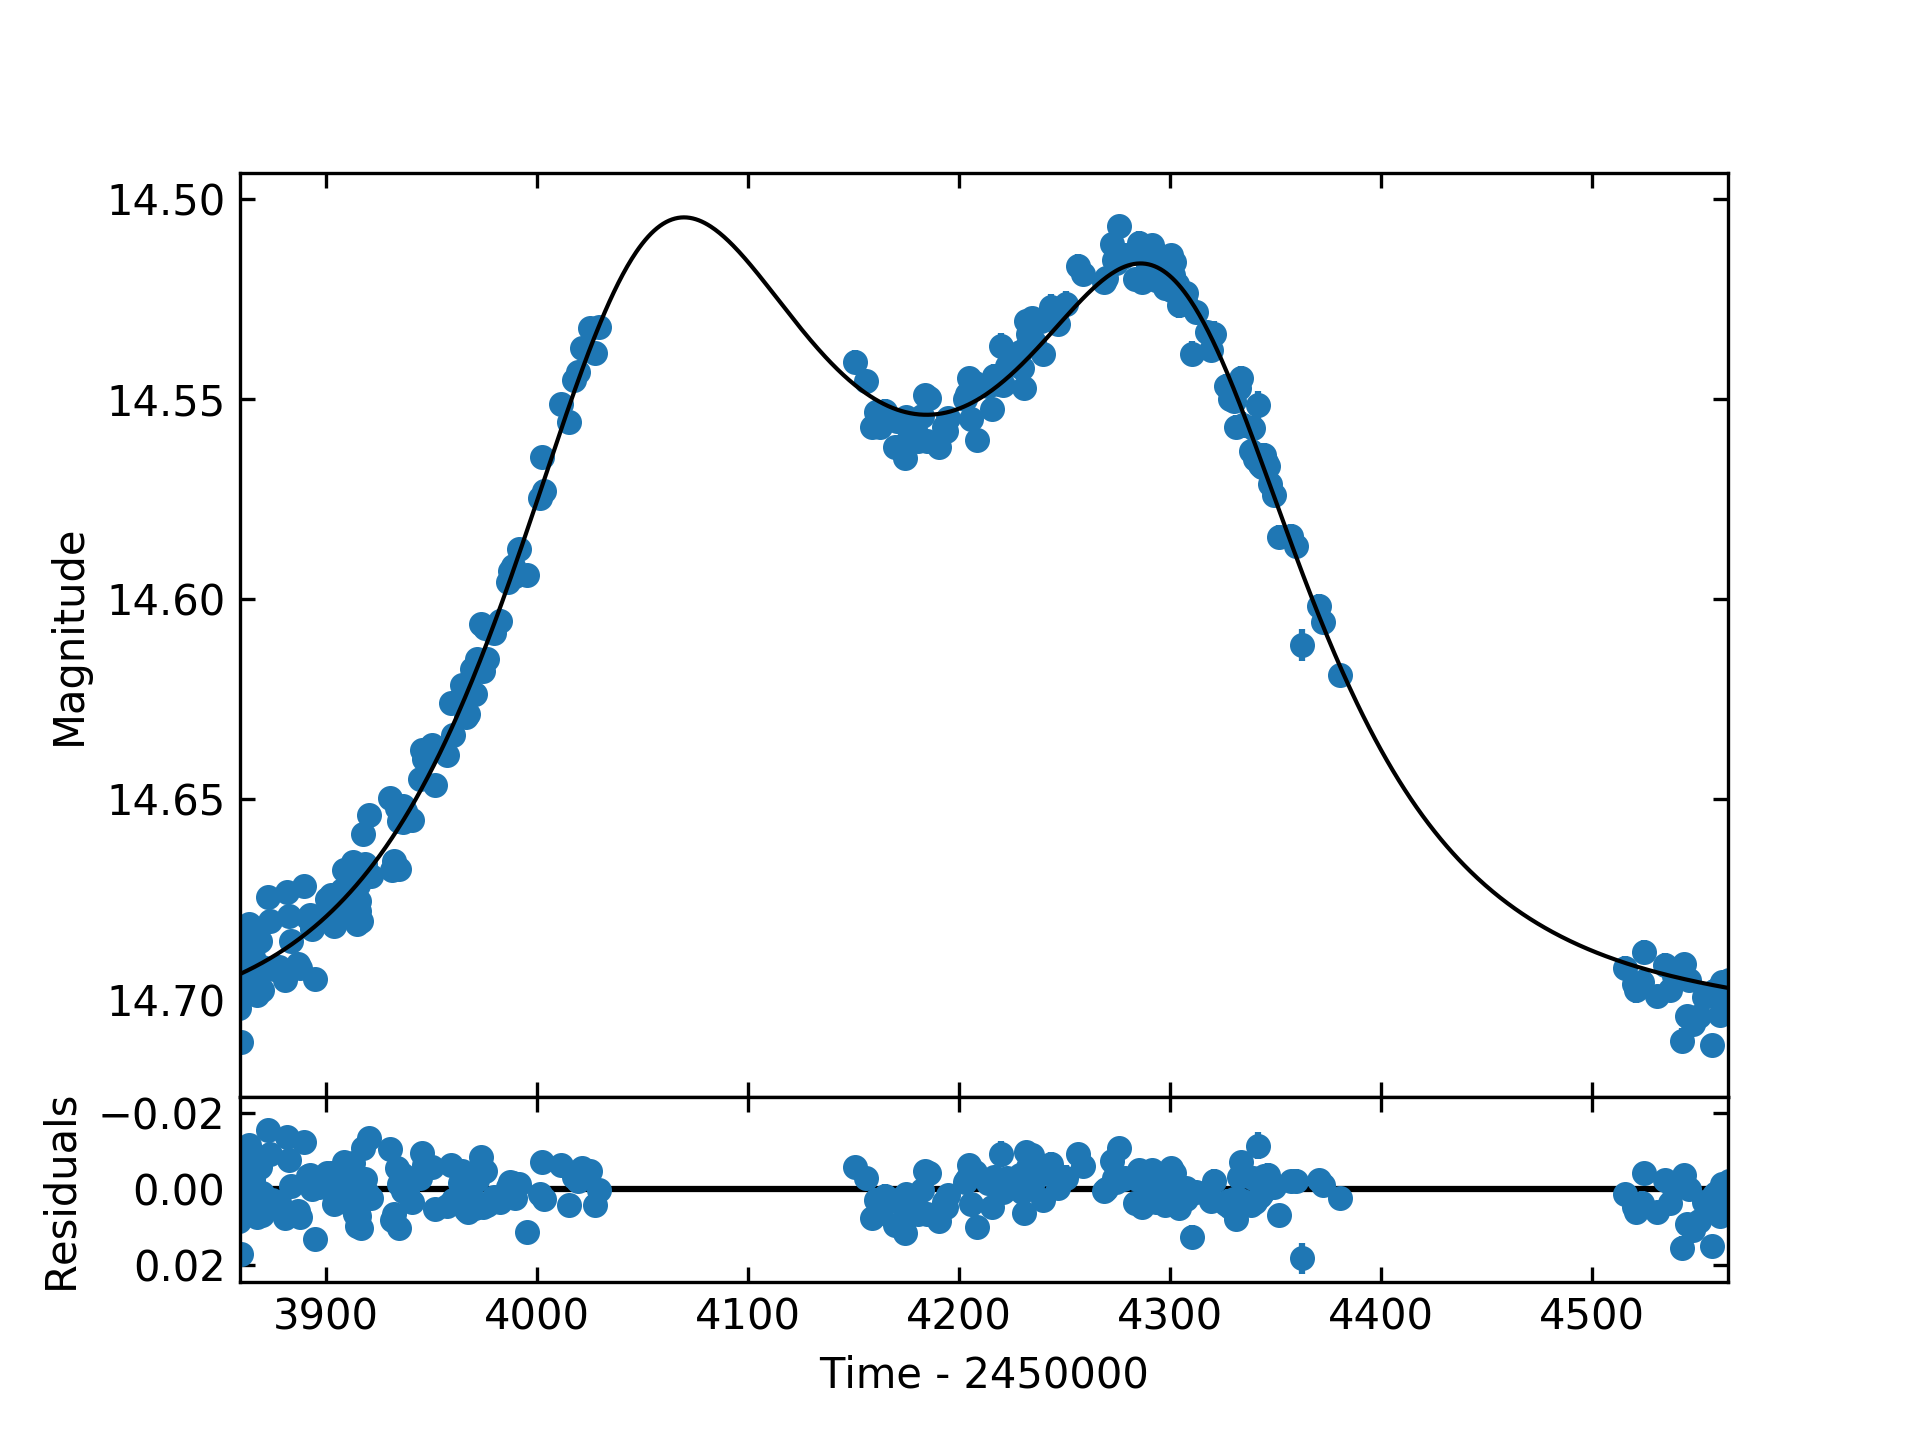
\includegraphics[width = \textwidth]{../sim30/xallarap/png/PAR-06-noaver.dat.10.png}
                \caption*{\tiny{PAR-06.10}}
            \end{figure}
        \end{column}
    \end{columns}
\end{frame}

\section{Modelowanie mikrosoczewkowania}
\subsection{MulensModel}
\begin{frame}
    \begin{columns}
        \begin{column}{0.5\linewidth}
            \emph{Mulens Model} \cite{MulensModel_paper}, to paczka służąca do modelowania zjawisk mikrosoczewkowania.
            Do dopasowania krzywej, używany jest algorytm MCMC (Próbkowanie Monte Carlo łańcuchami Markowa).

        \end{column}

        \begin{column}{0.5\linewidth}
            \begin{figure}
                
\includegraphics[width = \textwidth]{logoMM_crop_4_372x260.png}
            \end{figure}
        \end{column}
    \end{columns}
\end{frame}

\section{Rezultaty}

\begin{frame}{Opis projektu}
    59 zjawisk wykazujących dominujący wpływ paralaksy(?), z przeglądu OGLE-III (Wyrzykowski et al. 2016 \cite{Basis_paper}).

    \bigskip
    \bigskip

    A co jeśli źródło jest w układzie podwójnym?
\end{frame}

\begin{frame}{Porównanie modeli}
    \begin{table}[h]
        \centering
        \begin{tabularx}{\linewidth}{X r r}
            \toprule
            Nazwa  & $\Delta\chi^2$           & $\chi^2 _{Paraxall}$ \\
            \midrule
            PAR-05 & \textcolor{orange}{52.8} & 2360.0               \\
            PAR-06 & \textcolor{green}{304.5} & 4567.6               \\
            PAR-14 & \textcolor{orange}{37.3} & 7164.4               \\
            PAR-39 & \textcolor{green}{129.9} & 13677.8              \\
            PAR-57 & \textcolor{red}{59681.0} & 4335.8               \\
            PAR-58 & \textcolor{orange}{34.8} & 1087.9               \\
            PAR-59 & \textcolor{green}{124.1} & 2175.5               \\
            \bottomrule
        \end{tabularx}
    \end{table}

\end{frame}

\begin{frame}
    \centering
    \vspace{-0.3cm}
    \begin{columns}
        \begin{column}{0.5\linewidth}

            \begin{figure}
                \centering
                \begin{overpic}[width = \textwidth, keepaspectratio]{../sim30/parallax/png/PAR-06-noaver.dat-.png}
                    \put(40, 68){Parallax}
                \end{overpic}
            \end{figure}

        \end{column}
        \begin{column}{0.5\linewidth}

            \begin{figure}
                \centering
                \begin{overpic}[width = \textwidth, keepaspectratio]{../sim30/xallarap/png/PAR-06-noaver.dat.10.png}
                    \put(40, 68){Xallarap}
                \end{overpic}
            \end{figure}

        \end{column}
    \end{columns}

    \begin{figure}
        \centering
        \begin{overpic}[width = 0.5\textwidth, keepaspectratio]{../sim30/paraxall/png/PAR-06-noaver.dat-.png}
            \put(20, 68){ Parallax + Xallarap}
        \end{overpic}
    \end{figure}

\end{frame}

\begin{frame}{Wyniki}
    \centering
    \large{PAR-06}
    \begin{tabularx}{\linewidth}{Xr}
        \toprule
        Parametr                      & wartość                         \\
        \midrule
        $t_0 [d]$                     & $2454179.345_{-5.95 } ^{+7.17}$ \\
        $u_0 $                        & $-0.722_{-0.05 } ^{+0.05}$      \\
        $t_E [d]$                     & $203.621_{-7.99 } ^{+8.04}$     \\
        $\pi_{EN}$                    & $-0.014_{-0.02 } ^{+0.02}$      \\
        $\pi_{EE}$                    & $-0.035_{-0.01 } ^{+0.01}$      \\
        $\xi_{\text{period}} [d]$     & $392.271_{-3.58 } ^{+3.46}$     \\
        $\xi_{\text{semimajor axis}}$ & $0.154_{-0.02 } ^{+0.01}$       \\
        \bottomrule
    \end{tabularx}
\end{frame}

\begin{frame}{Kontynuacje badań}
    \centering
    \begin{tabular}{rrr}
        \toprule
               & (Wyrzykowski et at. 2016 \cite{Basis_paper}) & My                     \\
        Nazwa  & $M [M_{\odot}]$                              & $M_{lens} [M_{\odot}]$ \\
        \midrule
        PAR-05 & $3.3^{+2.7}_{-1.5}$                          & ?                      \\
        PAR-06 & $1.0^{+1.3}_{-0.5}$                          & ?                      \\
        PAR-14 & $0.2^{+0.3}_{-0.1}$                          & ?                      \\
        PAR-39 & $2.2^{+1.5}_{-1.1}$                          & ?                      \\
        PAR-57 & -                                            & ?                      \\
        PAR-58 & -                                            & ?                      \\
        PAR-59 & -                                            & ?                      \\
        \bottomrule
    \end{tabular}

\end{frame}

\begin{frame}{Kontynuacje badań}
    \begin{itemize}
        \item Wyznaczenie masy soczewek, dla których nasz model jest lepszy od modelu z paralaksą.
        \item Ponowne wymodelowanie zjawisk, w celu zmniejszenia niepewności.
        \item Zbadanie wpływu innych efektów na model (np. soczewka potrójna).
    \end{itemize}
\end{frame}

\begin{frame}{Bibliografia}

    \printbibliography
    \nocite{*}
\end{frame}

\end{document}